% Template for PLoS
% Version 1.0 January 2009
%
% To compile to pdf, run:
% latex plos.template
% bibtex plos.template
% latex plos.template
% latex plos.template
% dvipdf plos.template

\documentclass[10pt]{article}

% amsmath package, useful for mathematical formulas
\usepackage{amsmath}
% amssymb package, useful for mathematical symbols
\usepackage{amssymb}

% graphicx package, useful for including eps and pdf graphics
% include graphics with the command \includegraphics
\usepackage{graphicx}

% cite package, to clean up citations in the main text. Do not remove.
\usepackage{cite}

\usepackage{color} 

% Use doublespacing - comment out for single spacing
\usepackage{setspace} 
\doublespacing


% Text layout
\topmargin 0.0cm
\oddsidemargin 0.5cm
\evensidemargin 0.5cm
\textwidth 16cm 
\textheight 21cm

% Bold the 'Figure #' in the caption and separate it with a period
% Captions will be left justified
\usepackage[labelfont=bf,labelsep=period,justification=raggedright]{caption}

% Use the PLoS provided bibtex style
\bibliographystyle{plos2009}

% Remove brackets from numbering in List of References
\makeatletter
\renewcommand{\@biblabel}[1]{\quad#1.}
\makeatother


% Leave date blank
\date{}

\pagestyle{myheadings}
%% ** EDIT HERE **


%% ** EDIT HERE **
%% PLEASE INCLUDE ALL MACROS BELOW

%% END MACROS SECTION

\begin{document}

% Title must be 150 characters or less
\begin{flushleft}
{\Large
\textbf{Title}
}
%
% XXX
%
% VISUALIZING THE SPACE OF HYPERPARAMETERS IN NEURAL NETWORKS
% 
% LARGE-SCALE NETWORK TRAINING FOR EMPIRICAL ANALYSIS OF NEURAL NET PARAMETERS
%
% VISUALIZING HOW NEURAL NETWORKS LEARN
%
% VISUALIZING THE ENTIRE SPACE OF NEURAL NETWORK HYPER-PARAMETERS
%
% VISUSALIZING HOW NEURAL NETWORKS LEARN THROUGH LARGE-SCALE NETWORK TRAINING
%
% VISUALIZING HOW NEURAL NETWORK HYPER-PARAMETERS CHANGE LEARNING
%
% VISUALIZING HOW HYPER-PARAMETERS AFFECT LEARNING IN NEURAL NETWORKS
%
% Insert Author names, affiliations and corresponding author email.
\\
Christopher Olah$^{1,\ast}$, 

Michael A. Nielsen$^{2}$
\\
\bf{1} Hacklab Toronto, 170a Baldwin Street, Toronto, Ontario, Canada
\\
\bf{2} 2/120 Christie Street, Toronto, Ontario, Canada
\\
$\ast$ E-mail: colah@thielfellowship.org

\end{flushleft}

% Please keep the abstract between 250 and 300 words
\section*{Abstract}

% Please keep the Author Summary between 150 and 200 words
% Use first person. PLoS ONE authors please skip this step. 
% Author Summary not valid for PLoS ONE submissions.   
\section*{Author Summary}

\section*{Introduction}

%
% the trouble with neural nets
%
Artificial neural networks are a powerful machine learning technique
which achieve excellent results for many pattern recognition problems
(e.g. KSH, Ng, Seide, Dahl, Schmidhuber, Bengio on Maxout).  But while
powerful, they can be difficult to train, and performance often
depends sensitively on the choice of hyper-parameters for the neural
network.  Picking these hyper-parameters can be an art-form, often
involving considerable trial and error based on hard-to-describe
heuristics. (XXX - It'd be nice to have refs). Casual users of neural
networks sometimes get poor results for a problem they expect to be
soluble by their network.  At that point, they face a conundrum: are
the poor results because of some easily-fixed issue with the
hyper-parameters, or is there some deeper obstacle?  Because of these
concerns some people advocate sticking with less finicky methods such
as support vector machines and random forests.

%
% what we do in this paper: broad picture
%
In this paper, we use clusters of graphics processing units (GPUs) to
train more than 100,000 neural nets.  This lets us systematically
explore hyper-parameter space, and to develop vivid visualizations and
animations showing how the network learns for different choices of
hyper-parameters.  From these visualizations we extract several
heuristic rules of thumb for choosing neural network hyper-parameters.

%
% the flavour
%
To convey the type of experiments we do and the results we obtain,
consider the graph in Figure~\label{fig:example}.  This graph shows
the performance of a single neural network architecture on a
particular image recognition task.  The important thing is that
performance is shown for a very large number of different training
configurations, all with the same architecture.  In particular, the
$x$ and $y$ axes are two important hyper-parameters for the neural
network (details to be explained later).  So we've trained $40 \times
40 = 1,600$ neural nets, for $40$ different choices of the first
hyper-parameter, and $40$ different choices of the second
hyper-parameter.  The intensity of colour at the corresponding point
on the graph represents how well the neural network performs: dark is
poor performance, light is good performance.  By examining a
judiciously selected set of these graphs we will deduce heuristic
rules for choosing hyper-parameters.

%
\begin{figure}[!ht]
\begin{center}
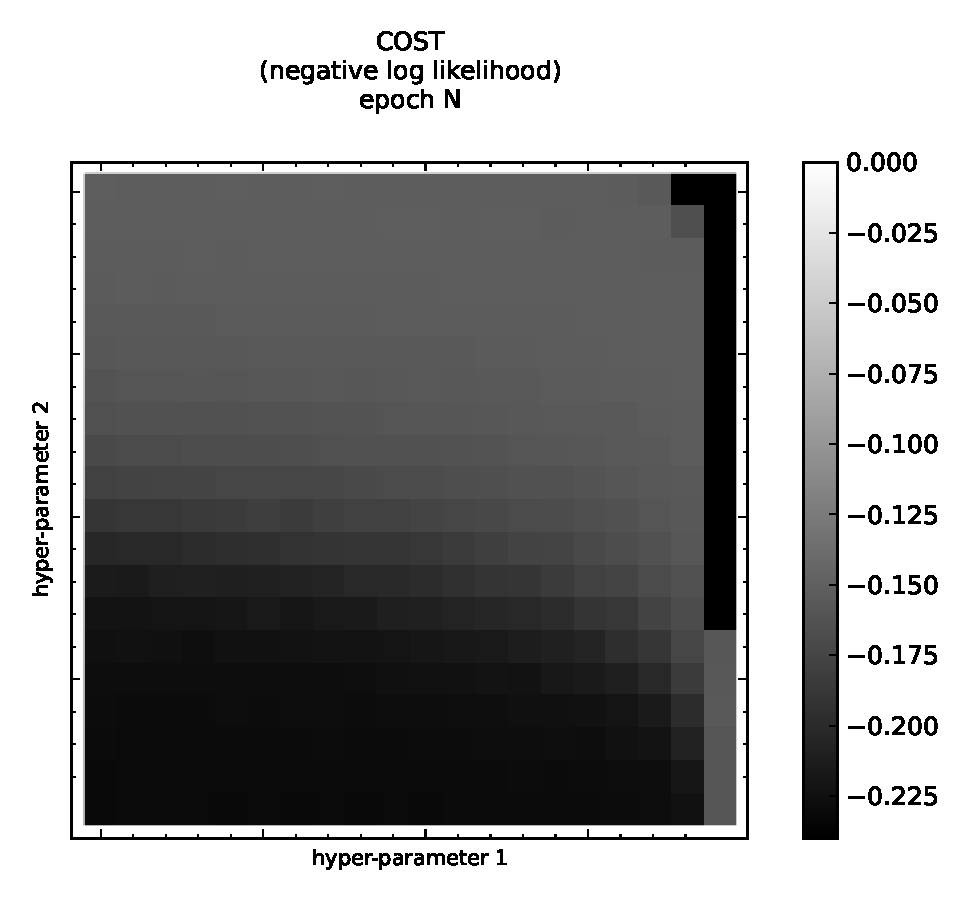
\includegraphics[width=4in]{plots/example.eps}
\end{center}
\caption{ {\bf The performance of a single neural network architecture
    on a particular image recognition task}.  Lower cost represents
  better performance.  See the text for details.}
\label{fig:example}
\end{figure}

%XXX --- sigmoid, 20 hidden unit, friction versus learning rate.
%Labels: hyper-parameter 1.  hyper-parameter 2.  Cost: nice gradient
%bar thing.  Title(ish): After training epoch 3.



%
% expanding on the type of results we get
%
The last paragraph describes our basic approach.  In fact, we will
obtain not just single graphs, but entire animations showing how
neural networks improve as they are trained.  This lets us see in a
vivid way how the networks improve for different choices of
hyper-parameters.  In this journal we cannot embed the animations
directly, but will instead show sequences of graphs.  This is nearly
as good as the animations to convey the results.  The Supporting
Information contains the full animations.  We also develop several
other similar video-based visualization techniques, but this example
already conveys the general flavour.

%
% The problem with the conventional approach to heuristics paragraph
%
There's a kind of folk wisdom of artificial neural networks --- a
collection of commonly-used heuristics that experts use to set
hyper-parameters.  Such heuristics have been collected in volumes such
as XXX (NNTOTD I, and II), as well as in many individual papers.
These heuristics have led to many successes, and often really do
improve neural network performance.

%
% What can go wrong as a result
%
However, while such heuristics can be useful, they are often based on
the investigation of a small number of networks.  The problem with
using such small-scale anecdotal evidence is that people may come to
believe heuristics that are misleading or even wrong.  A heuristic may
hold for some particular examples, but not in other circumstances.
One can see this in the large number of papers which introduce a new
technique, and provide evidence that technique is superior for some
class of problems, but then other users of neural nets do not find any
benefits to the technique, outside extremely similar circumstances.

%
% example of where we can _see_ what's going wrong
%
Another problem is that even a heuristic which is literally true may
have significant caveats.  For example, there has been much recent
interest in rectified linear units (ReLUs, $max(0,x)$,
\cite{Glorot2010a,Nair2010a,Jarrett2009a}), a type of artificial
neuron which appears to learn faster than other common types of
neuron, such as sigmoid and tanh units. \cite{Krizhevsky2012a} Our
results confirm that this is often the case, but, as we shall see, it
is also often much harder to find hyper-parameters so ReLUs learn
quickly.  We are able to provide a compelling visualization
demonstrating this, and also to precisely quantify how much harder it
is to optimize with ReLUs.

%
% how we approach this problem
%
In our approach we plot animations of two-dimensional slices of
hyper-parameter space.  This lets us explicitly see how different
combinations of hyper-parameters affect performance.  Done
judiciously, this gives us a more comprehensive viewpoint from which
to derive heuristics, and more robust conclusions than in the
conventional approach described above.  Of course, these 2-d slices do
not provide us with a comprehensive point of view, because other
hyper-parameters are being held fixed.  Furthermore, for any given
slice we cannot guarantee that any heuristics deduced will hold for
other choices of hyper-parameter.  However, we can build confidence by
plotting slices for several different choices of the other
hyper-parameters.  This visualization-based approach seems to be new
and complementary to prior work.

%
% complementary to Bayesian parameter optimization
%
In recent years there has been considerable focus on automated
procedures for finding hyper-parameters.  The simplest approaches are
box search (XXX cite) and variations.  More sophisticated methods are
now being developed, such as XXX, and Bayesian parameter optimization.
Encouraging recent results on Bayesian parameter optimization achieve
XXX.  However, to make Bayesian parameter optimization work well you
need good choices of prior distribution on the hyper-parameters.  The
results and approach we develop in this paper can help identify good
priors, and build confidence that a choice of priors is well motivated
(or, perhaps, should be modified).

%
% the curse of dimensionality: we're not claiming to escape it
%
Of course, our approach remains subject to the curse of
dimensionality.  Hyper-parameter space is high dimensional, and it's
inherently difficult to build up a comprehensive picture, even using
2-dimensional slices.  However, this statement of course also applies
to anyone trying to build up an understanding by hand-tuning single
hyper-parameters, trying to find just the ``right'' setting.  Our goal
is not to obtain a complete picture.  Instead, it's merely to develop
general (but partial) methods for understanding the structure of
hyper-parameter space.  It is a clear win to map out an entire 2-d
slice of hyper-parameter space at a fine-grained resolution, helping
us to better understand the relationships between those two
hyper-parameters.

% Results and Discussion can be combined.
\section*{Results and Discussion}

\subsection*{Experiments}

\subsubsection*{Learning rate versus momentum coefficient}

The learning algorithm we will use for our all experiments is
mini-batch stochastic gradient descent using momentum (XXX --- cite).
In our first set of experiments, described in this section, we
investigate learning as a function of two hyper-parameters: the
learning rate and the momentum coefficient.  Our experiments will lead
us to conjecture several heuristic relationships between these two
hyper-parameters.

Later sections will present similar experiments using other pairs of
hyper-parameters.  The next section gives a high-level overview of the
entire sequence of experiments, and discusses why different pairs of
hyper-parameters were chosen for investigation.  We could, of course,
have begun with that high-level overview.  However, since our
experiments are somewhat unusual in the neural networks literature, it
makes sense to start first with concrete results, since they will make
the high-level overview easier to understand.

Our experiments were performed using three neural network
architectures: a net with a single hidden layer containing 20 hidden
units; a net with a single hidden layer containing 40 hidden units;
and a net with two hidden layers, containing 40 and 20 hidden units,
respectively. All networks have an input layer with a neuron
corresponding to each pixel in the input image, in the case of the
grey-scale images in MNIST, and three neurons, corresponding to the
RGB intensities, for the images in CIFAR-10.  There is also an output
layer with a neuron for each classification label (ten for all the
datasets we use), followed by a softmax layer.

The experiments made use of four separate activation functions: the
sigmoid (i.e., logistic), hyperbolic tangent (tanh), rectified linear
units (ReLU), and softplus \cite{Glorot2010a,Dugas2001a}.  These
activation functions were applied throughout the network.

The experiments were performed using the MNIST (LeCun et al. (1998))
and CIFAR-10 (Krizhevsky (2009)) data sets.  These are well-known
labelled training sets used for image recognition.  Training was
performed using a negative log-likelihood cost function.

The graph in Figure~\ref{fig:mnist_basic} shows the behaviour of 1,600
neural networks when trained on the MNIST data for six epochs. These
correspond to 40 choices of the learning rate and 40 choices of the
momentum coefficient, for a total of 1,600 = 40 $\times$ 40 networks.

%
\begin{figure}[!ht]
\begin{center}
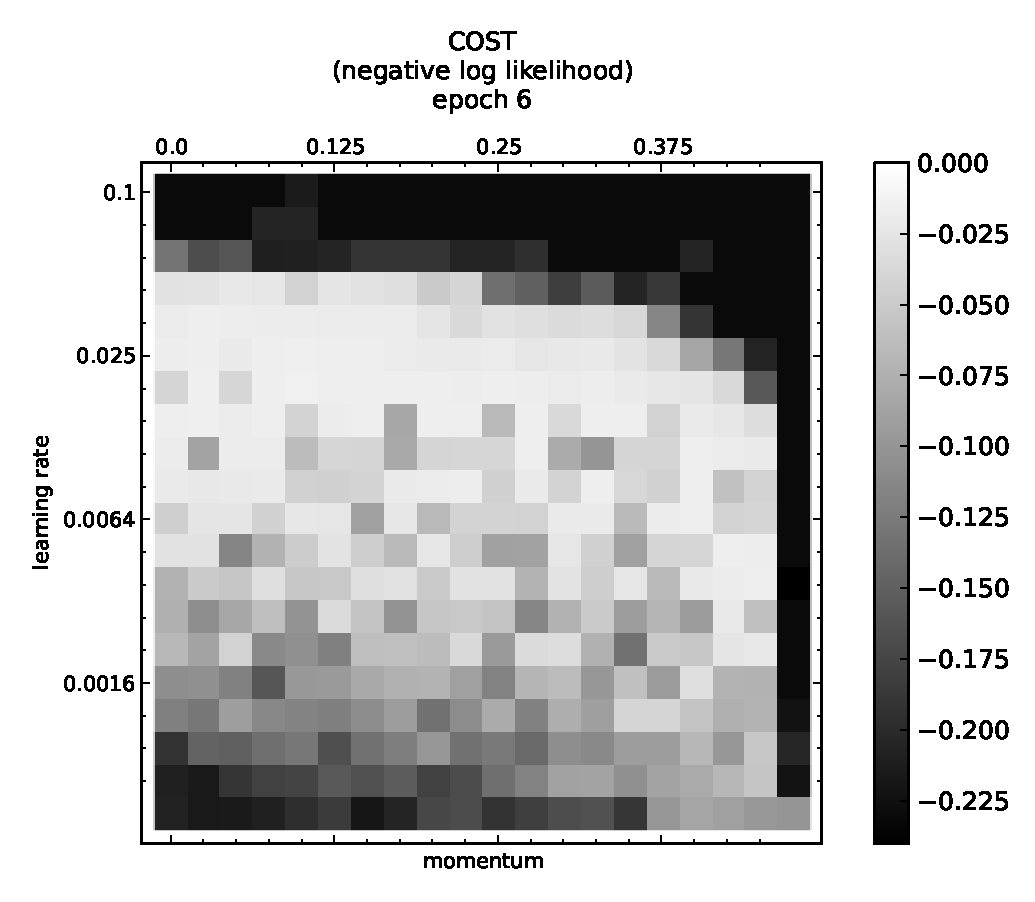
\includegraphics[width=4in]{plots/detailed/LF-20R10R-20T10-MNIST-6.eps}
\end{center}
\caption{ {\bf The behaviour of 1,600 neural networks when trained on
    the MNIST data for six epochs.}}
\label{fig:mnist_basic}
\end{figure}
%
% XXX --- This is currently a lie, we ony have 400 = 20 x 20.
%
% XXX - check: what do people actually do in terms of exploring momentum?
% Take a a look at four or five papers.
%
% XXX - ideally, learning rate labels should be in factors of 10.
%
% XXX - we want to comment on the power law.  Replot with log momentum?
%
% XXX - Range: 10**-4 to 1?  SOme other range?

To generate this graph we sampled 40 different values for the momentum
coefficient, ranging uniformly over 0.0 to 1.0.  This sampling process
reflects the way many researchers informally explore to find suitable
values for the momentum coefficient, often trying a number of values,
0.0, 0.1, 0.2, 0.3, and then perhaps adjusting slightly once they've
found a good first approximation.

While we sampled uniformly for momentum, we instead sampled uniformly
on the logarithm of the learning rate.  This reflects the way many
researchers informally explore to find suitable values for the
learning rate, often trying a number of values, 0.1, 0.01, 0.001, and
so on.  A similar but more fine-grained approach is often used in
systematic grid searches.  We use a maximum value of 1.0 XXX for the
learning rate, since in all our MNIST experiments the nets did not
appear to be learning anything when the learning rate was that high.
We use a minimum value of 0.0001 XXX for the learning rate.  With
these choices our range for the learning rate includes values which
have been used in much of the prior literature on MNIST.

A natural question is why we vary the learning rate while holding the
number of epochs constant.  Naively, this seems unnatural, since the
distance traversed by the stochastic gradient descent algorithm will
be proportional to the learning rate times the number of training
epochs.

However, in practice, with fixed computational resources, the number
of epochs we can train for is roughly a constant.  And so the question
that confronts someone looking to choose good hyper-parameters is how
to choose the learning rate which gives the best results after a fixed
number of epochs.

There's an additional heuristic justification for this practice. When
searching for a local minimum, we first pass through a transient phase
in which the stochastic gradient descent algorithm tries to get near
that minimum as quickly as possible.  The higher the learning rate the
fewer epochs required.  But once that transient phase is over it is no
longer the speed of movement which matters.  If, in our examples, this
happens very early on --- say after one or fewer epochs --- then the
naive argument given above completely breaks down, and it makes sense
to study learning rate and momentum as independent variables, with the
total training time fixed.  We cannot defend this argument, since we
have not precisely defined transience, and thus cannot say whether we
exit this regime quickly in our examples.  However, we mention the
argument since some informal testing suggests that we do exit the
transient phase quickly over much of our hyper-parameter space.

% We don't actually know how to define transient, or what smoking gun
% to look for.  It might be interesting to look at a quantity like g_n
% . g_{n+1} / norms, where g_n is the gradient at the nth iteration.
% This probably starts out positive, and then transitions to zero at
% some point --- that's a good start on a definition of a transient
% phase.
%
% XXX --- OLD VERSION OF THE ABOVE ARGUMENT: The following is an
% alternative answer to the above question We don't have the evidence
% to support that we're in this post-transient phase (although we
% suspect we are for most of the parameters plotted)
%
% Wouldn't it make more sense to vary the number of epochs so the
% product with the learning rate was a constant?  This argument is
% correct during an initial transient phase in which we're trying to
% get into the neighbourhood of a reasonable solution to the cost
% optimization problem.  But it's no longer correct when exploring the
% microstructure of the fitness landscape near that neighborhood.

A weakness of the approach is that we only train for 6 epochs.  This
was chosen because it was computationally feasible given our computing
resources.  With more computing power it would be desirable to train
for more epochs.  We do note that the classification accuracies we
obtained after 6 epochs (using the best hyper-parameters) are
comparable to those obtained historically for similar architectures.
Note also that recent research XXX suggests the value of going to very
large numbers of epochs (on the order of $10^3$), and using an
annealing schedule for learning which ultimately results in very low
learning rates.  We do not investigate these possibilities here,
although they suggest natural questions for the future.

% XXX --- Some interesting speculation here.  We haven't actually done it.
% 
% Why did we go for n epochs (where n is whatever it is?)  Combination
% of two answers: (1) Here's our evidence that we're near asymptoting
% --- to obtain this, do curve fitting to estimate what the long-run
% cost will be, assume that the cost after 3 epochs is given by $c_1 +
% c_2 * exp(c_3 t)$, where t is the time; (2) Computationally, that's as
% much as we could do.  Shoot for n = 5 or 6 or so.  Note that we need
% to validate the use of the exponential as an approximation for the
% long-run cost.  We ignore first 3 epochs due to possible transients.

The following table summarizes our MNIST results by providing a graph,
like the previous one, for all architectures and all activation
functions. Each row corresponds to an activation function, and each
column to an architecture.  The architecture is indicated in the
column heading, e.g., the first column shows results with the 28
$\times$ 28 = 784 input units, 20 hidden units, and 10 output units.
The color scheme for cost and the axes are the same as in the previous
graph, but left unlabeled to avoid clutter.

\begin{tabular}{|c|c|c|c|}
        \hline
        & & Cost for the MNIST data & \\
        & & set after 6 epochs & \\
        \hline
         & 784-20-10 & 784-40-10 & 784-40-20-10\\ \hline
sigmoid 
        & 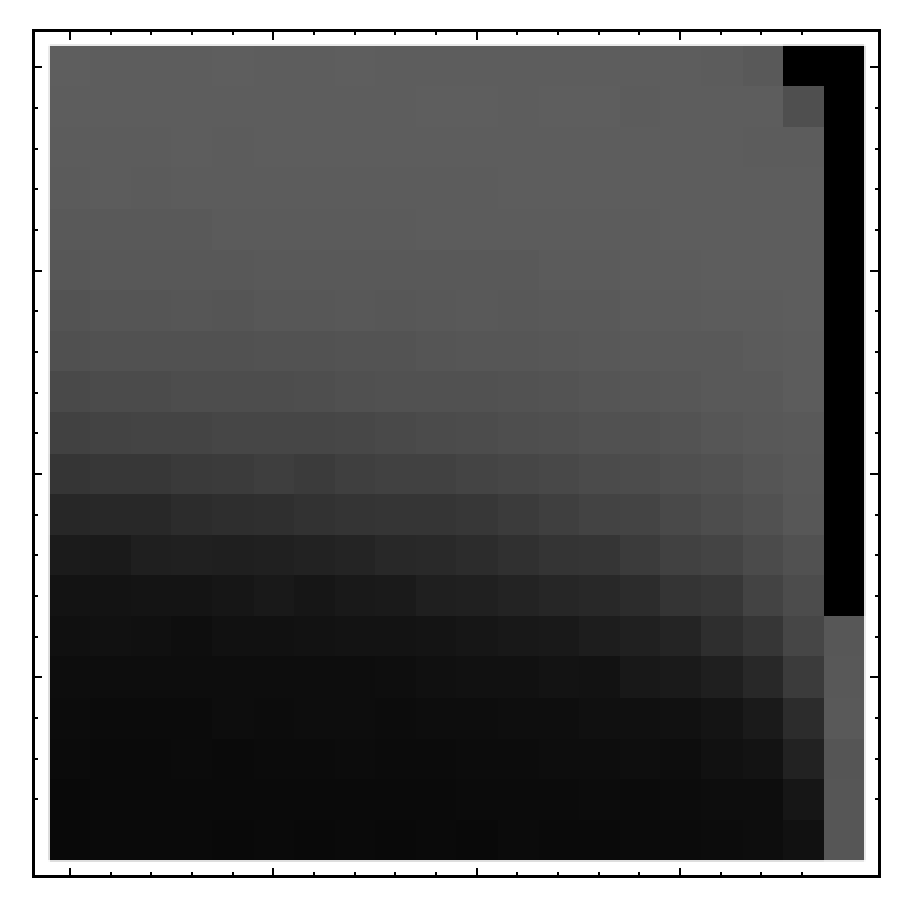
\includegraphics[scale=0.25]{plots/simple/LF-20S10S-20T10-MNIST-6.eps}
        & 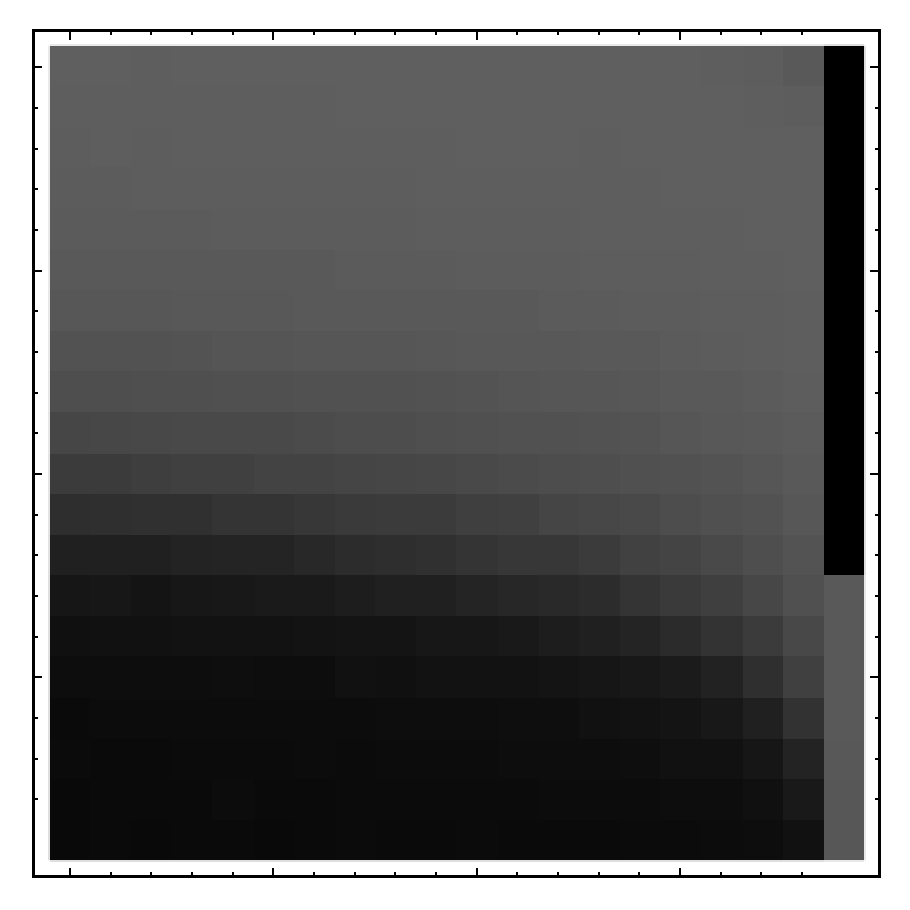
\includegraphics[scale=0.25]{plots/simple/LF-40S10S-20T10-MNIST-6.eps}
        & 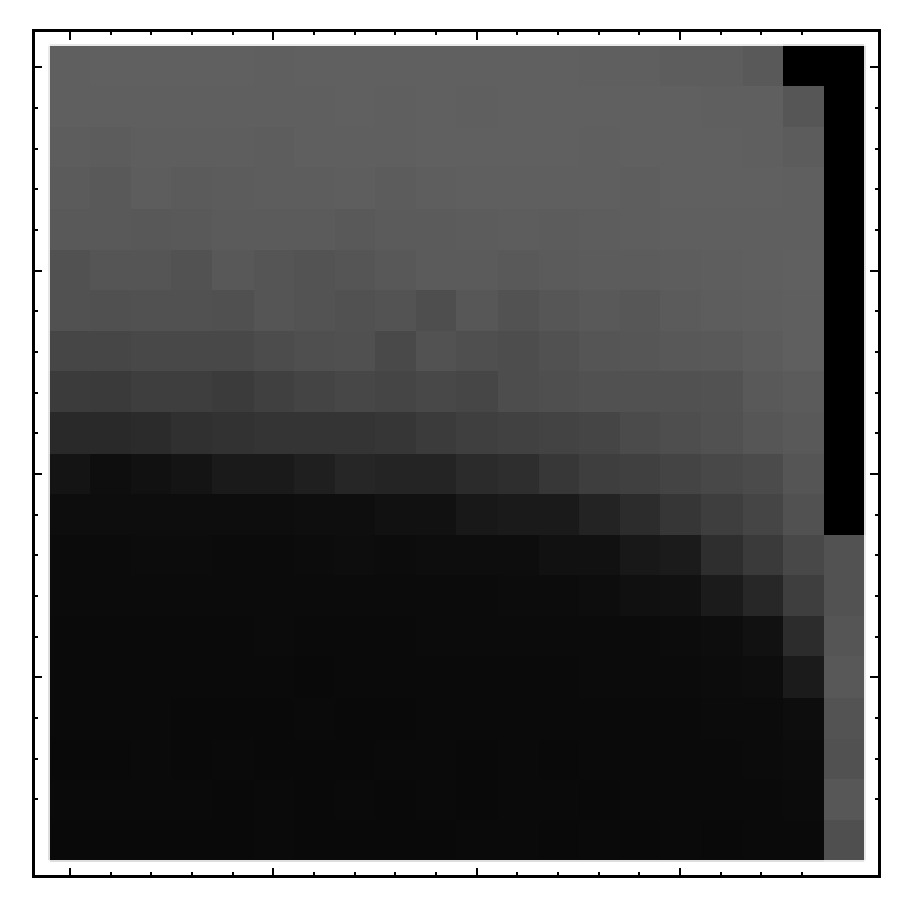
\includegraphics[scale=0.25]{plots/simple/LF-40S20S10S-20T10-MNIST-6.eps} \\ \hline
tanh
        & 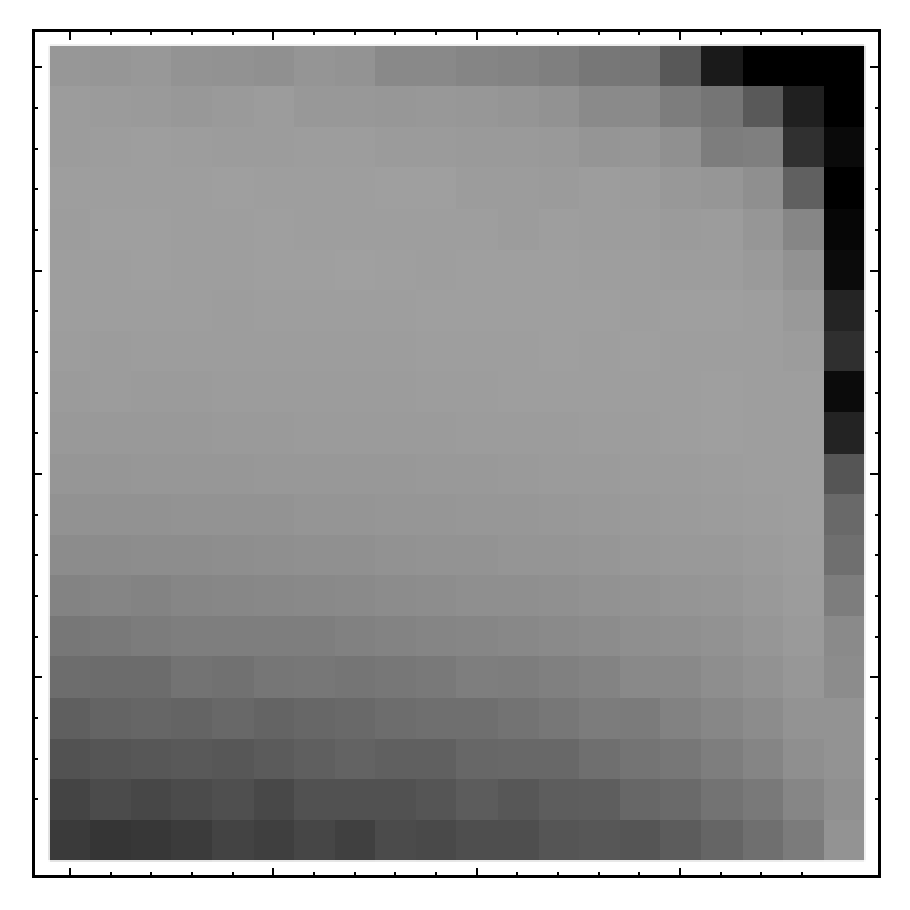
\includegraphics[scale=0.25]{plots/simple/LF-20T10T-20T10-MNIST-6.eps}
        & 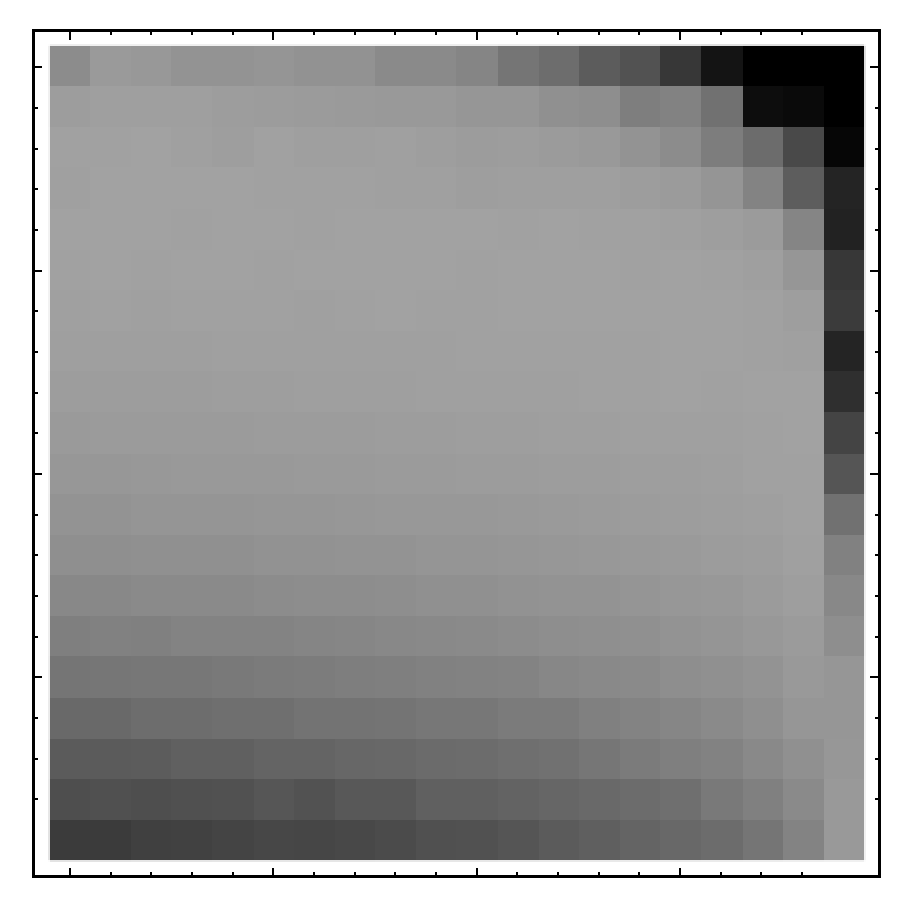
\includegraphics[scale=0.25]{plots/simple/LF-40T10T-20T10-MNIST-6.eps}
        & 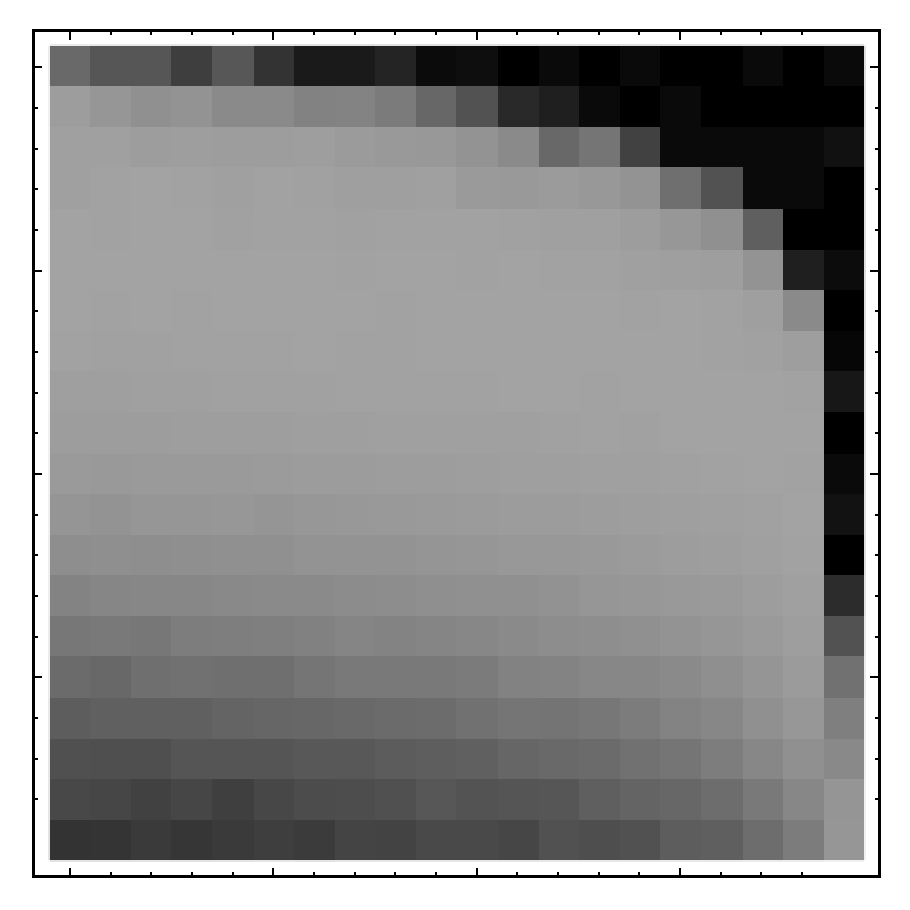
\includegraphics[scale=0.25]{plots/simple/LF-40T20T10T-20T10-MNIST-6.eps} \\ \hline
ReLU 
        & 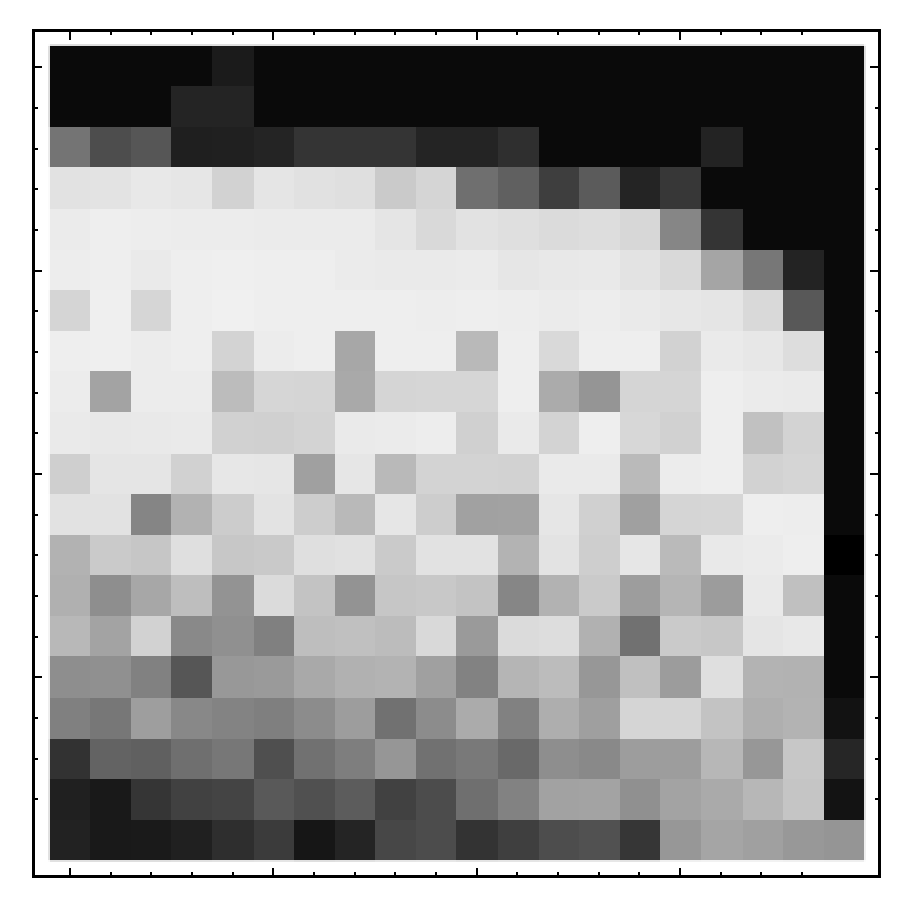
\includegraphics[scale=0.25]{plots/simple/LF-20R10R-20T10-MNIST-6.eps}
        & 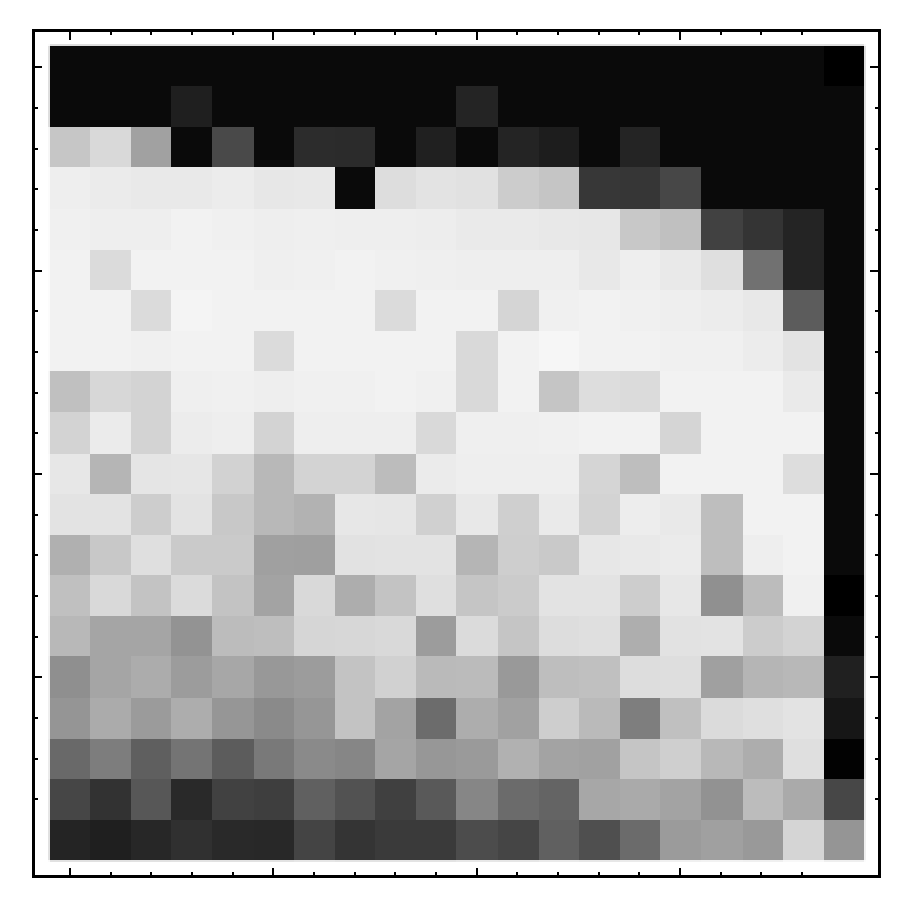
\includegraphics[scale=0.25]{plots/simple/LF-40R10R-20T10-MNIST-6.eps}
        & 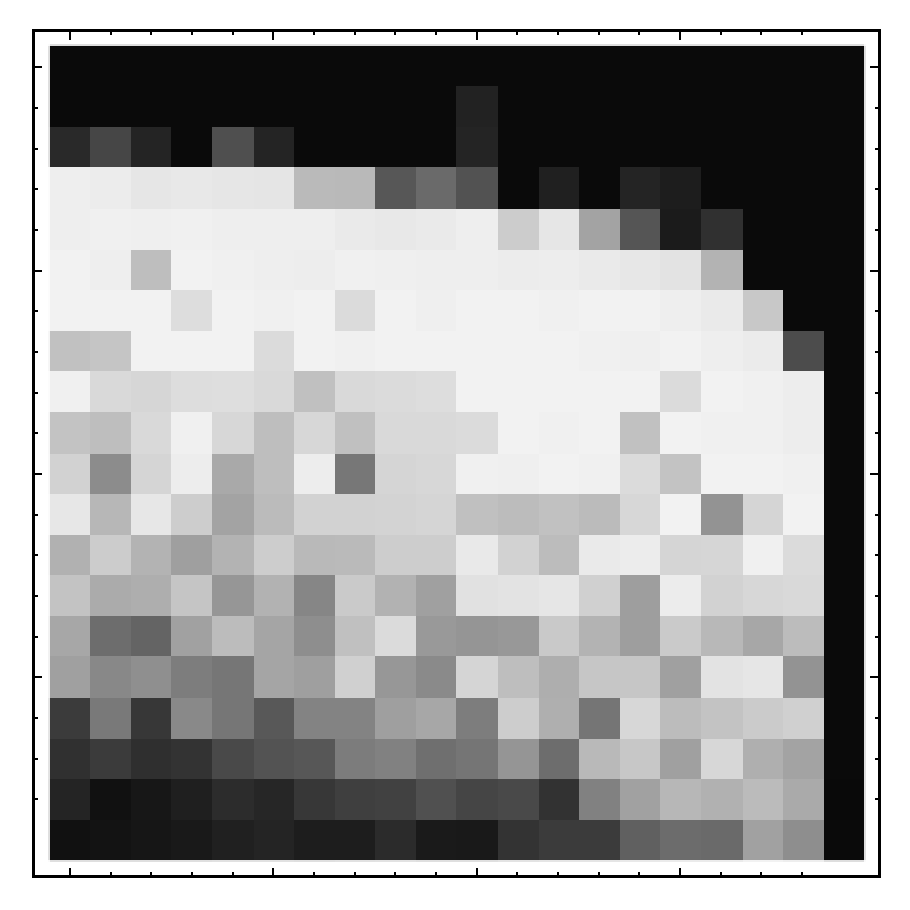
\includegraphics[scale=0.25]{plots/simple/LF-40R20R10R-20T10-MNIST-6.eps} \\ \hline
XXX softplus 
        & 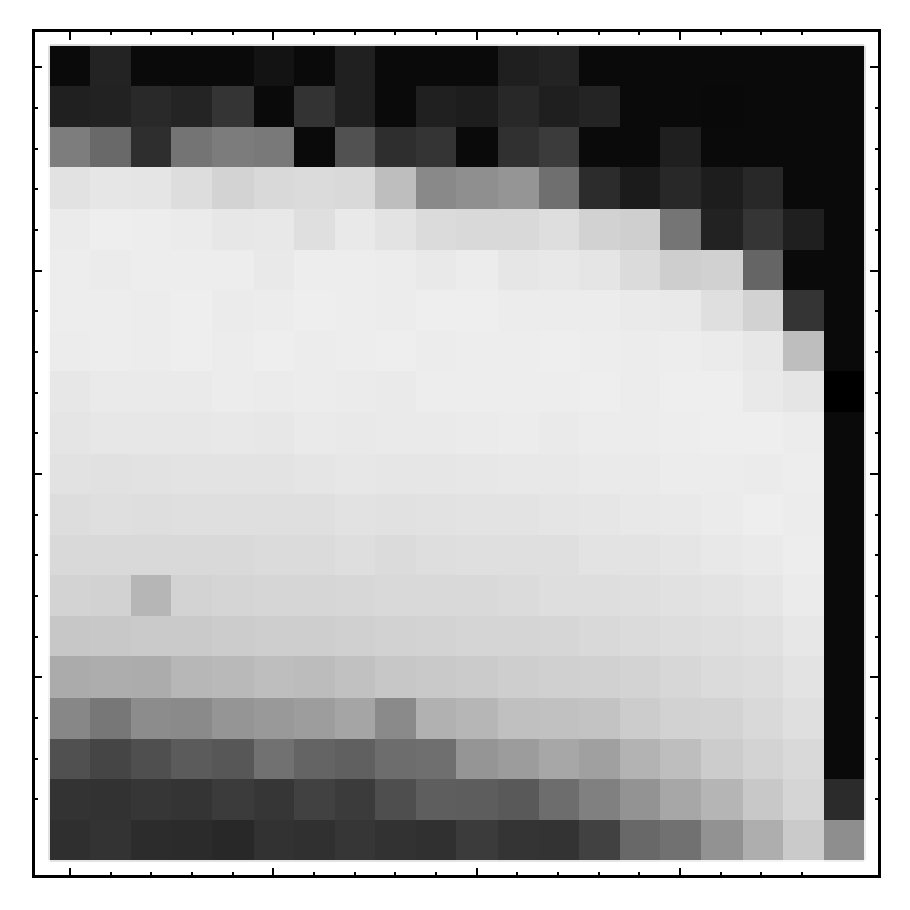
\includegraphics[scale=0.25]{plots/simple/LF-20B10B-20T10-MNIST-6.eps}
        & 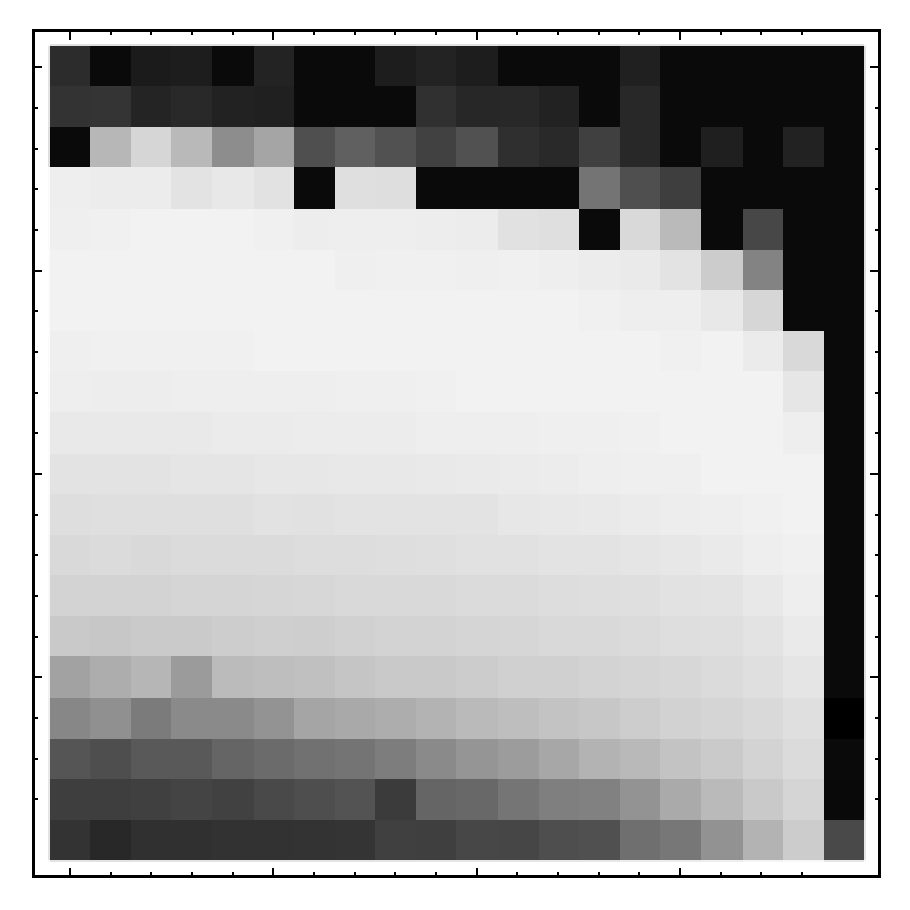
\includegraphics[scale=0.25]{plots/simple/LF-40B10B-20T10-MNIST-6.eps}
        & 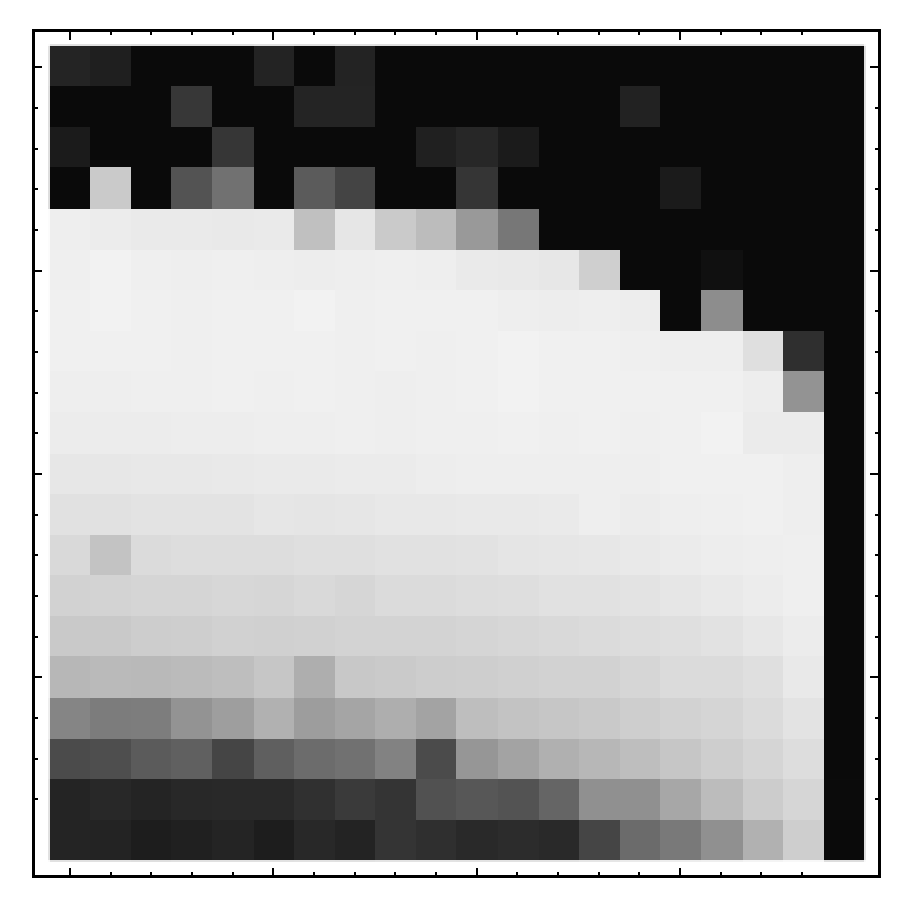
\includegraphics[scale=0.25]{plots/simple/LF-40B20B10B-20T10-MNIST-6.eps} \\ \hline
\end{tabular}

As before, all these graphs visualize cost after 6 epochs of
training. Animated versions of these graphs, showing how cost changes
over training, are provided in the supplementary material as Videos
S1-S12, along with the code that generates the videos.

We can summarize these results in another visualization, shown in
Figure~\label{fig:fraction}: (XXX - replot this without BReLu, fix
labels, do at epoch 6, use fraction not percent, change ``cost'' to
``cost threshold'') What this graph shows is the fraction of
hyper-parameters that achieve a cost below a given cost threshold,
plotted for several different activation functions.  So, for example,
let's look at the ReLU graph at a cost threshold of $0.05$.  We see
that the corresponding fraction is about $0.35$.  What this means is
that in our earlier ReLU experiments (fig.~XXX) about 35 percent of
the experiments achieved a cost below $0.05$.

\begin{figure}[!ht]
\begin{center}
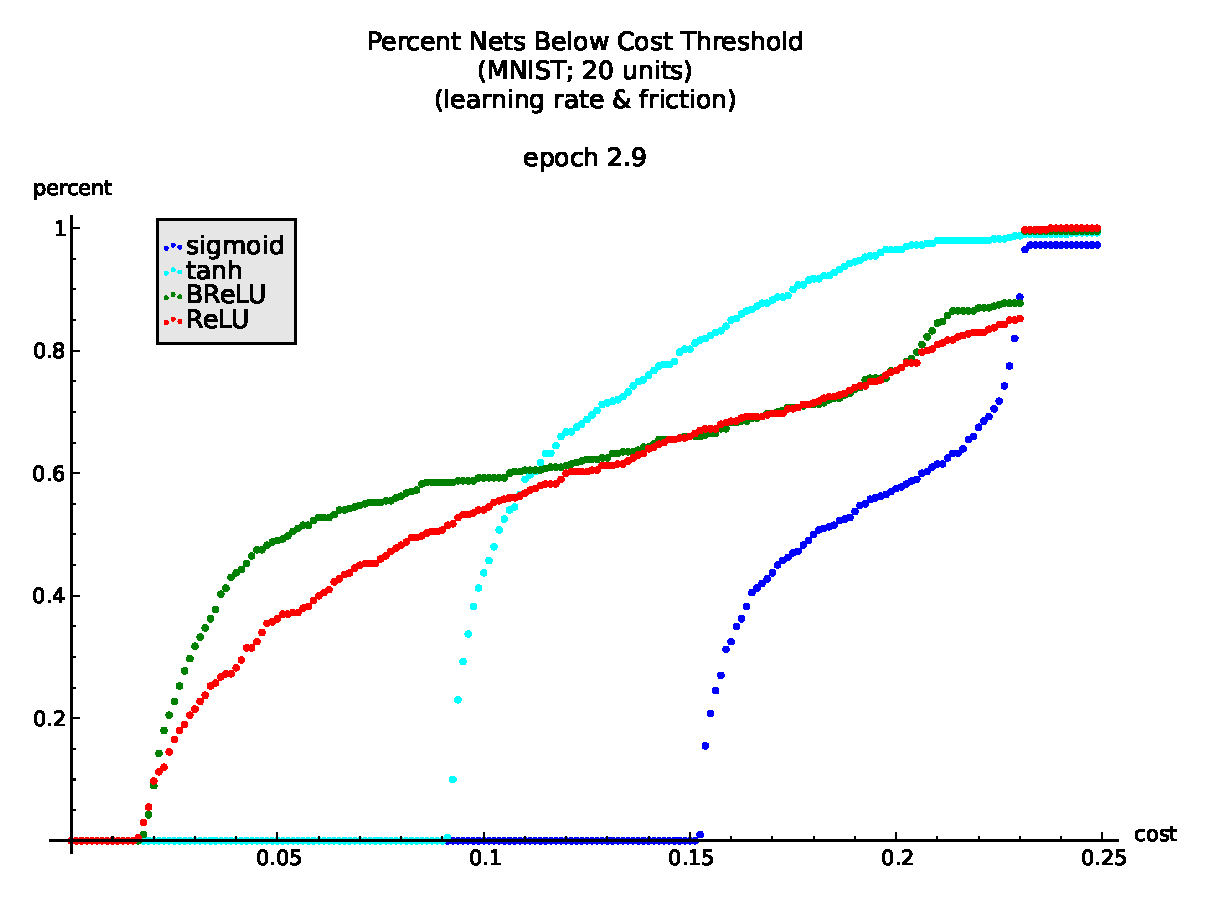
\includegraphics[width=4in]{plots/detailed/LF-20a10a-20T10-MNIST-3-percent.eps}
\end{center}
\caption{ {\bf The fraction of hyper-parameters achieving a cost below
    a given cost threshold.}}
\label{fig:fraction}
\end{figure}

We see that this graph quantifies not only how well a network does for
the best choice of hyper-parameters, but also how easy it is to tune.
We can see, for example, that ReLUs achieve slightly better best-case
performance than BReLUs (XXX--true for softplus?), but BReLUs are
significantly easier to tune to get near-to-best-case performance.

The above graph is static.  In Video S13 we show how the graph changes
as a function of training time.  For the particular case of MNIST and
the 20 hidden neuron architecture, the graph changes only a little
qualitatively over time.  Later, in our discussion of CIFAR-10, the
video will reveal striking qualitative changes in the performance of
the different activation functions.

The results above suggest a number of observations:

\textbf{Observation 1:} For near-optimal costs, softplus (XXX) has
many more good hyper-parameters in the momentum-learning rate space
than there are for other activation functions.

\textbf{Observation 2:} ReLU's best-case performance is better than
the tanh and sigmoid, and generally comparable to softplus, with the
better performance depending on the details of the architecture.  Our
results on softplus (XXX) suggest that some ReLUs are becoming
inactive (and thus stopping learning), which can be avoided with
softplus.

\textbf{Observation 3:} ReLUs have substantially more stochastic
behaviour.  They provide good best-case performance, but are sensitive
to small perturbations.  By contrast all our other activation
functions are much smoother.  This makes it easier to find relatively
stable solutions that won't just fall apart.  

Informally, people who work with large, deep ReLU-based convolutional
neural networks do not report this kind of instability (cite
Goodfellow, personal communication XXX).  However, so far as we know
this has not been quantitatively studied.  If the informal observation
is borne out then it would be interesting to understand the reasons
for this difference.

\textbf{Observation 4:} This is really a collection of closely-related
observations about the...

Consider again one of our earlier plots... XXX... Removing all the
structure from it we obtain... XXX.  Suppose we fix a given value of
momentum.  Then at what value or values of the learning rate do we
obtain the optimal cost?  A prior it seems possible that there might
be many possible values: XXX.  There might be regions, or even
multiple regions: XXX.  Our data suggest that in fact the cost is a
convex function of the learning rate, and that there is a single value
for the optimal learning rate.  Now, we can repeat this process for
other values of momentum, and, again, we find a single optimal value
for the corresponding learning rate.  So we can actually plot a graph
showing the optimal learning rate for each different momentum: XXX.
The shape of this graph is roughly the same for all activation
functions and architectures. qWhat is truly remarkable, however, is
that it seems that the optimal value for the cost is very nearly
independent of the value of the momentum.  To put it another way, if
we consider the values of (learning rate, momentum) which come near to
optimizing the cost, then they are approximated by a one-dimensional
curve: XXX.  The shape of this curve varies from thing to thing, but
is broadly consistent.  A priori, of course, this need not have been
the case.  It is perfectly possible that this near-optimizing set of
hyper-parameters have a very complex shape: XXX.  This has several
nice consequences.  First, cost is relatively insensitive to the
choice of momentum.  For practical purposes, setting momentum at 0 and
usually regular gradient descent seems to work about as well as with
the optimal value of momen tum.


Of course, our data does not in any sense confirm that these
observations hold generally, since the data used to suggest a
hypothesis cannot also be used to confirm it!  However, it does
suggest investigating these observations



CIFAR:

Note that the CIFAR results were only obtained for the net
architecture using 20 hidden units.

Note also that we weren't verifying a hypothesis.

\begin{figure}[!ht]
\begin{center}
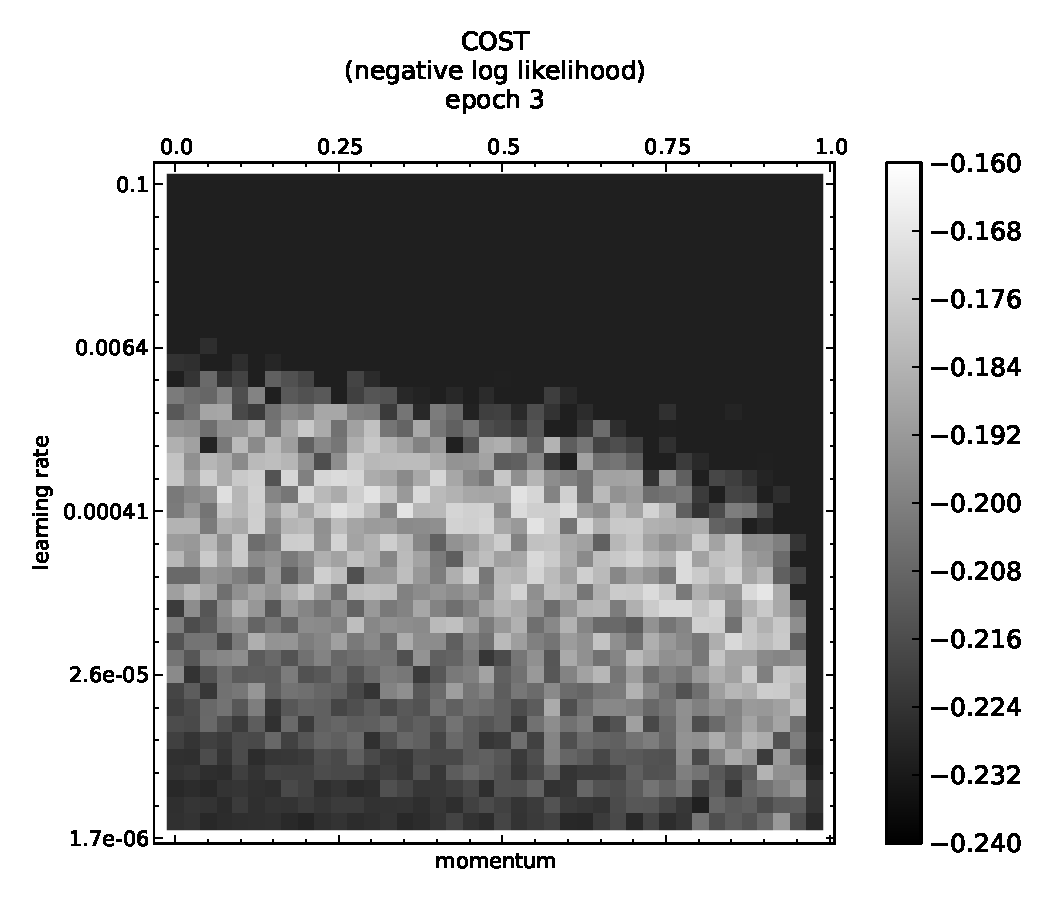
\includegraphics[width=4in]{plots/detailed/LF-20R10R-20T10-CIFAR-3.eps}
\end{center}
\caption{
{\bf Bold the first sentence.}  Rest of figure 2  caption.  Caption 
should be left justified, as specified by the options to the caption 
package.
}
\label{Figure_label}
\end{figure}

\begin{tabular}{|c|c|c|c|}
        \hline
        & & {\LARGE cost} & \\
        & & (CIFAR-10) & \\
        & & (negative log-likelihood) & \\
        & & (20-10-softmax) & \\
        \hline
         & 1 epoch & 2 epochs & 3 epochs\\ \hline
sigmoid 
        & 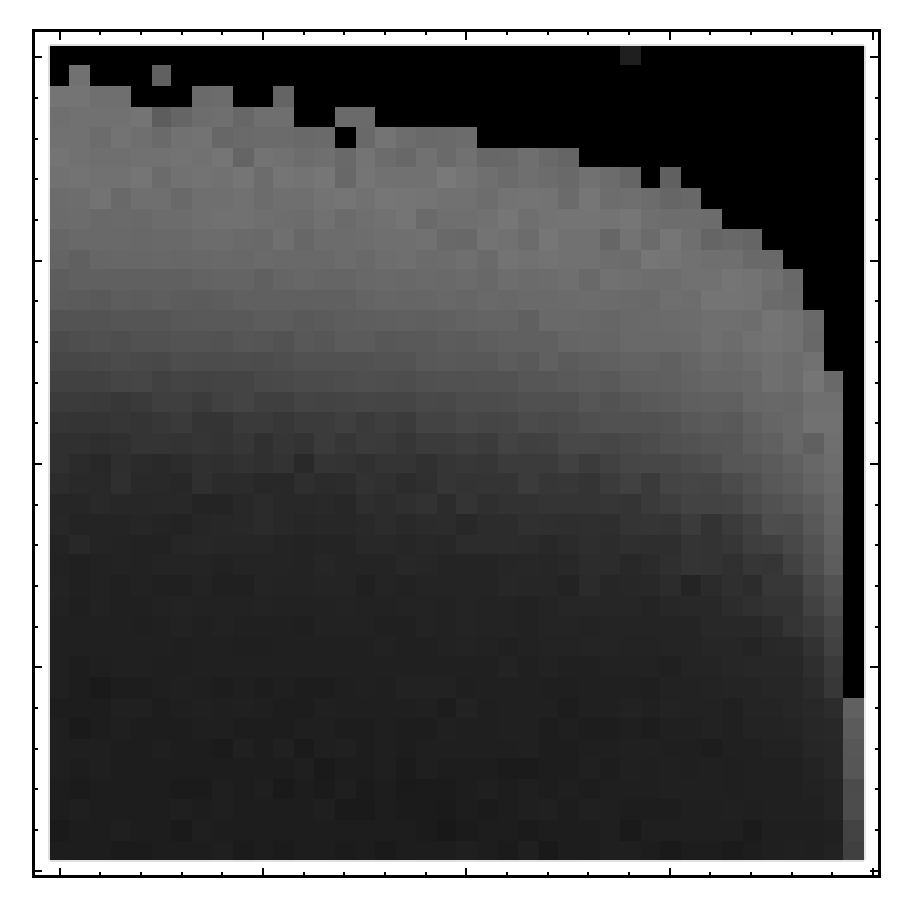
\includegraphics[scale=0.25]{plots/simple/LF-20S10S-20T10-CIFAR-1.eps}
        & 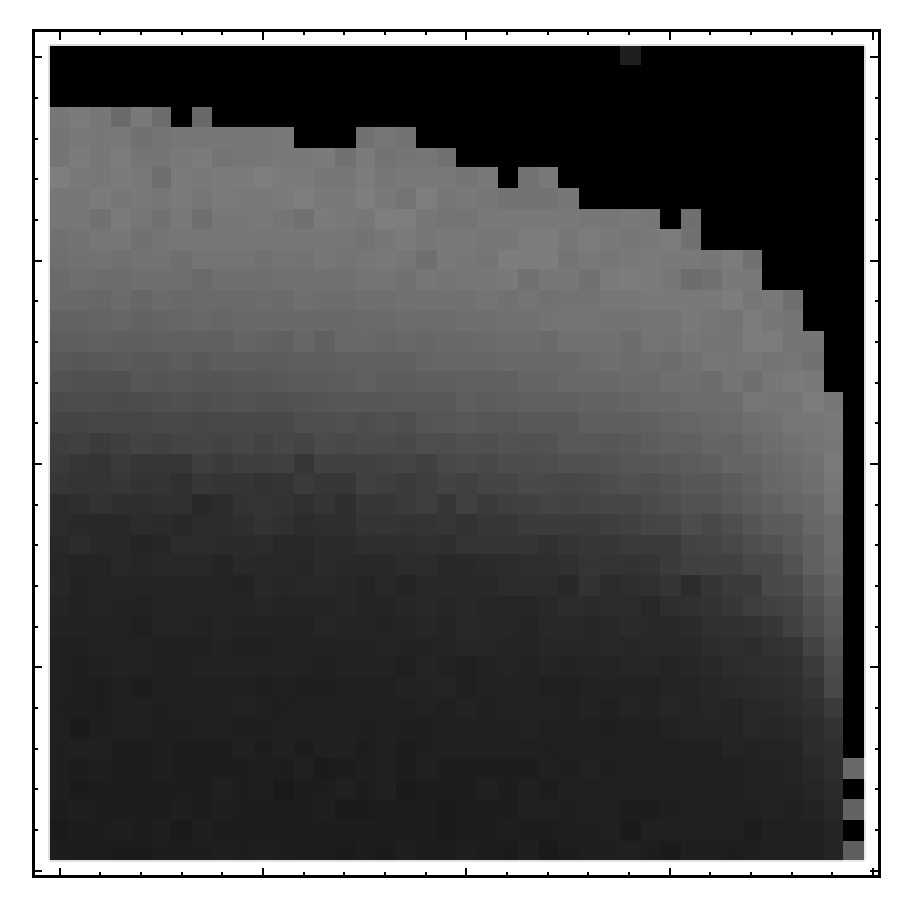
\includegraphics[scale=0.25]{plots/simple/LF-20S10S-20T10-CIFAR-2.eps}
        & 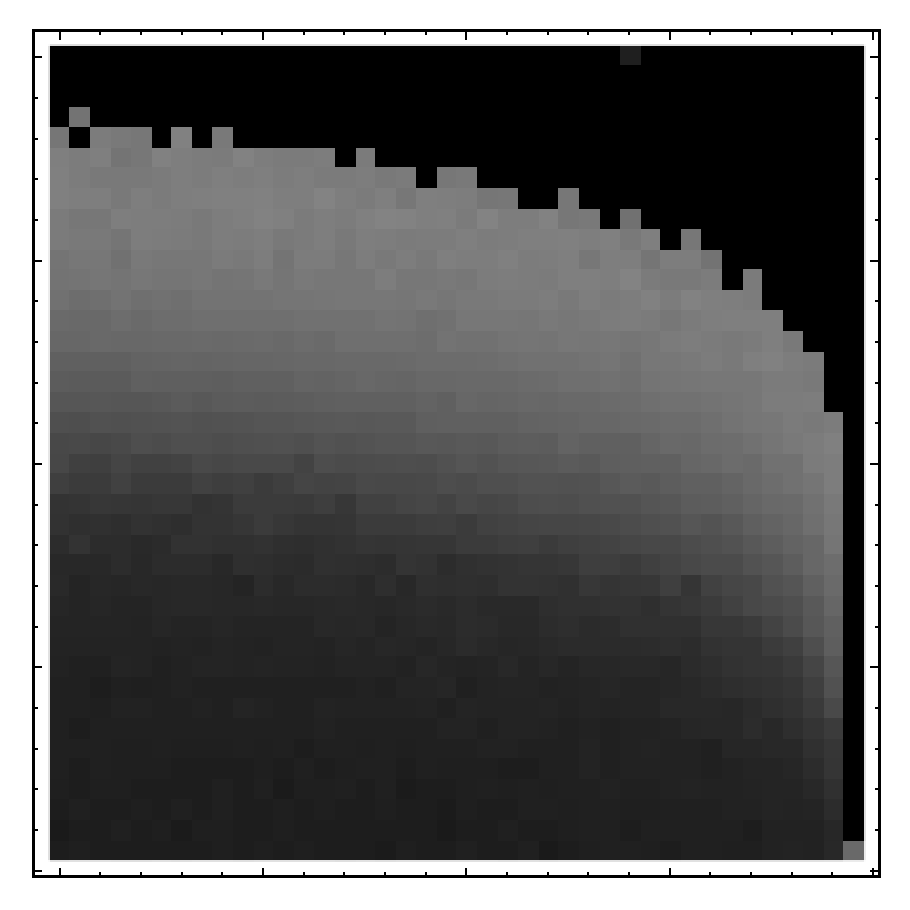
\includegraphics[scale=0.25]{plots/simple/LF-20S10S-20T10-CIFAR-3.eps} \\ \hline
tanh 
        & 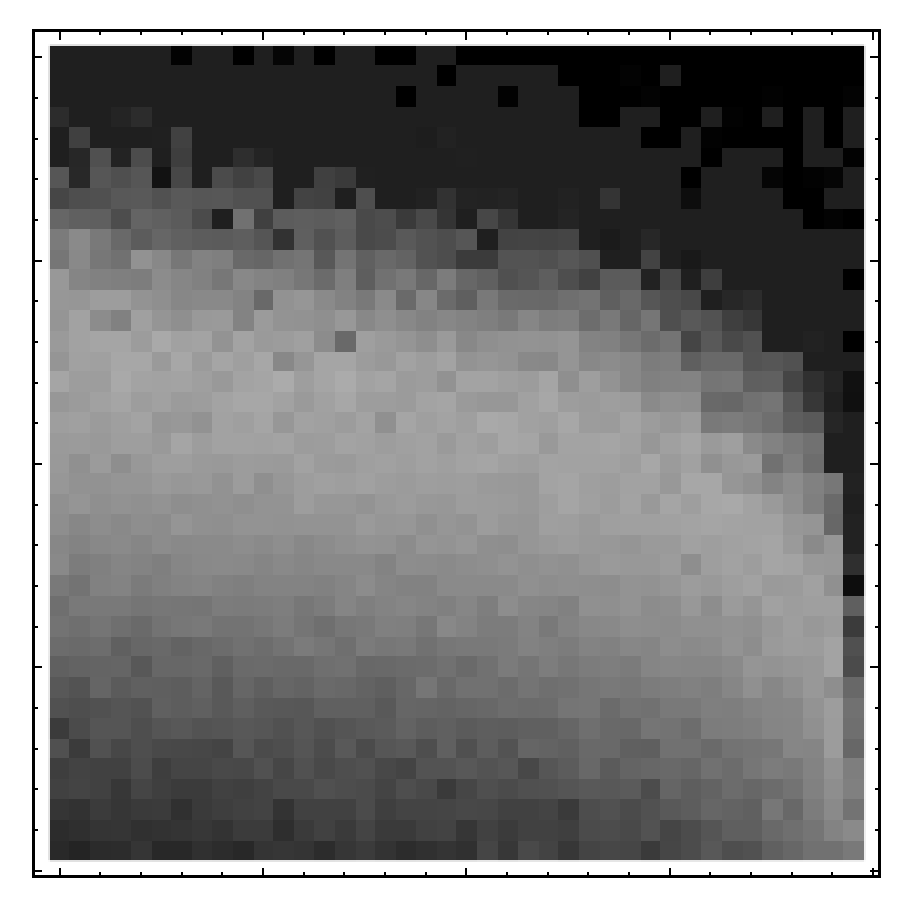
\includegraphics[scale=0.25]{plots/simple/LF-20T10T-20T10-CIFAR-1.eps}
        & 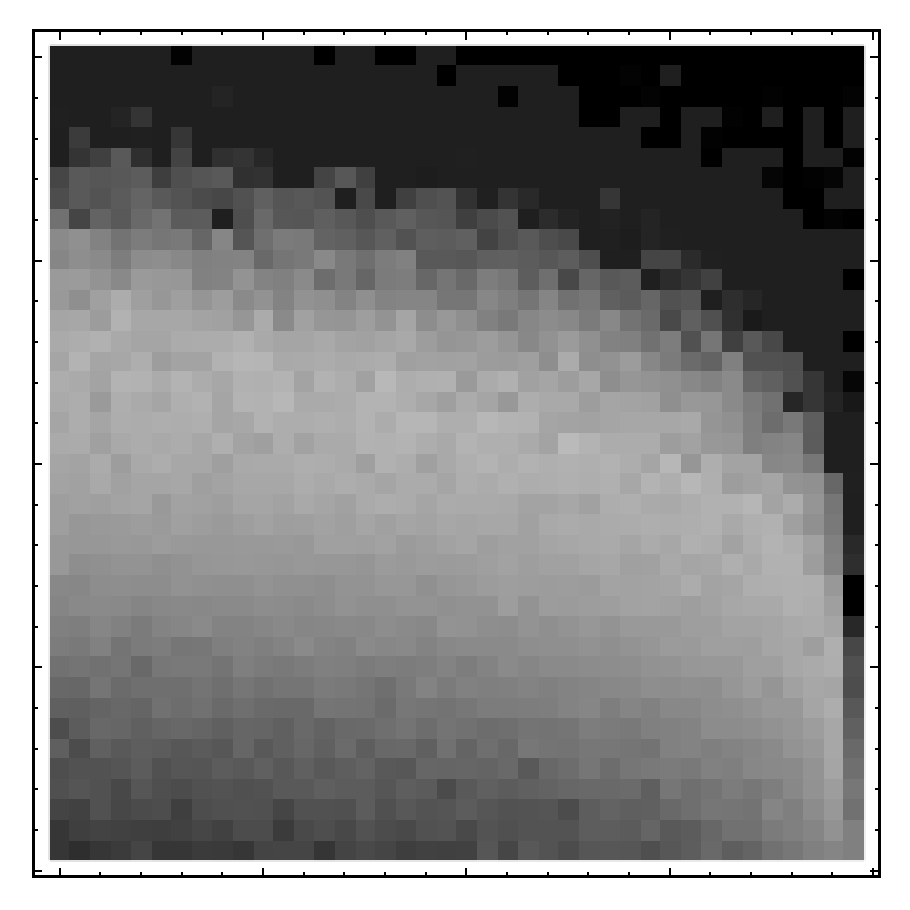
\includegraphics[scale=0.25]{plots/simple/LF-20T10T-20T10-CIFAR-2.eps}
        & 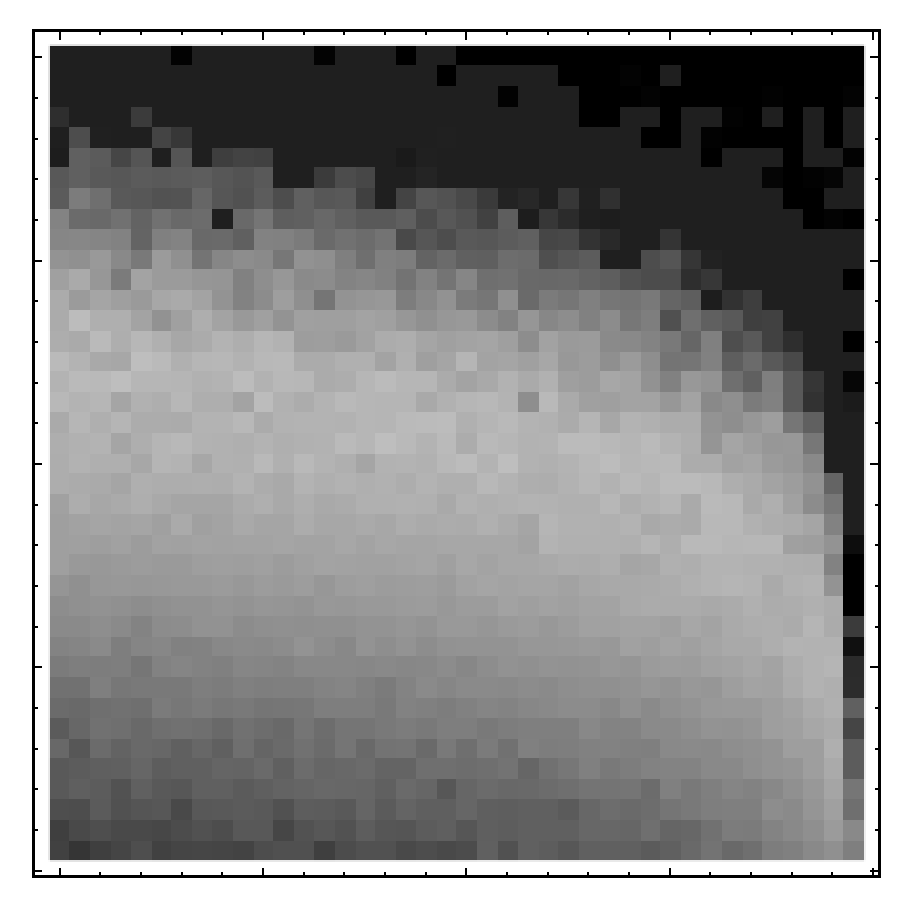
\includegraphics[scale=0.25]{plots/simple/LF-20T10T-20T10-CIFAR-3.eps} \\ \hline
ReLU 
        & 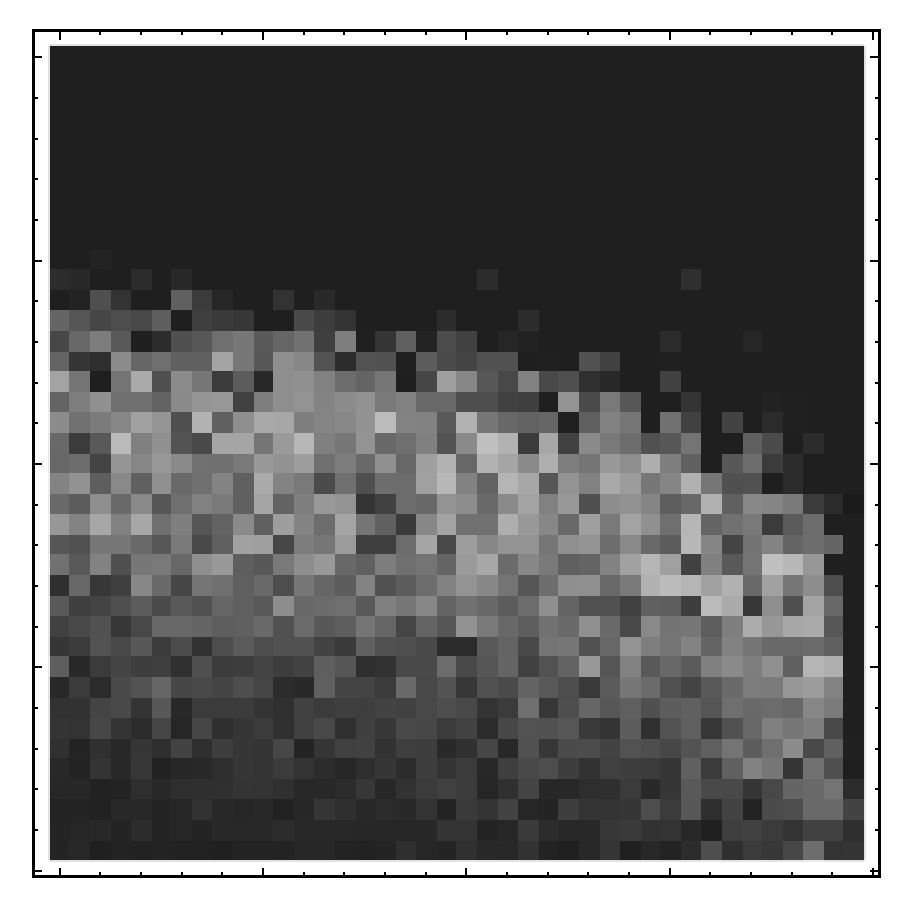
\includegraphics[scale=0.25]{plots/simple/LF-20R10R-20T10-CIFAR-1.eps}
        & 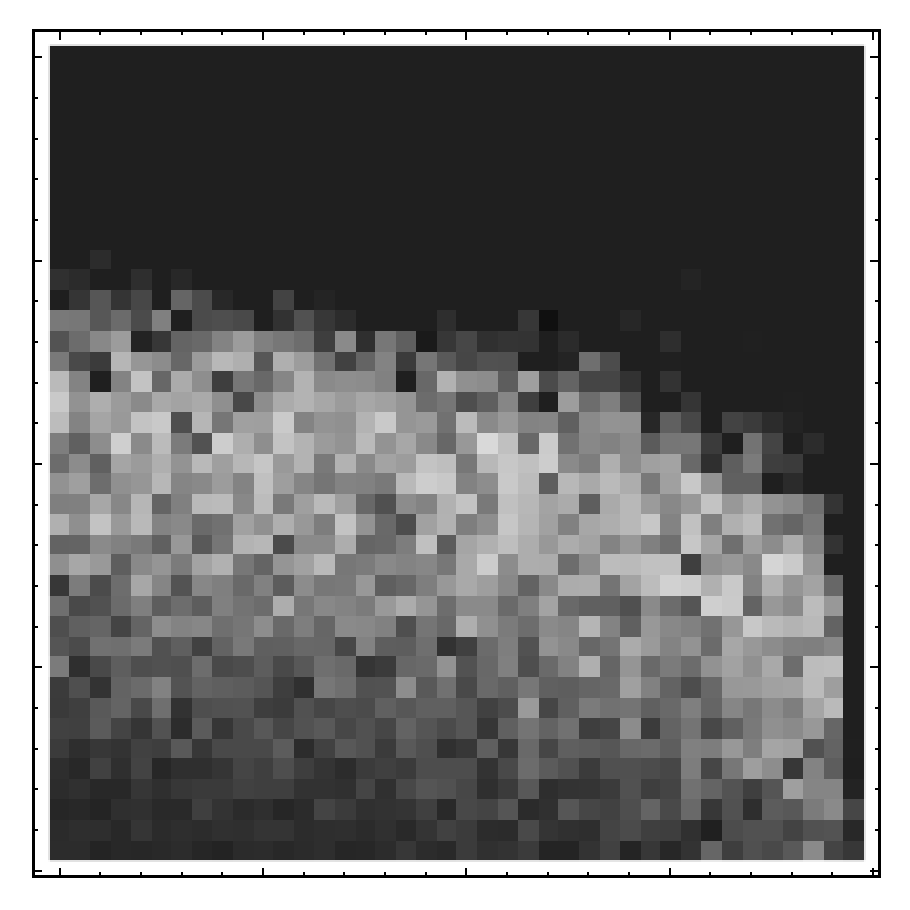
\includegraphics[scale=0.25]{plots/simple/LF-20R10R-20T10-CIFAR-2.eps}
        & 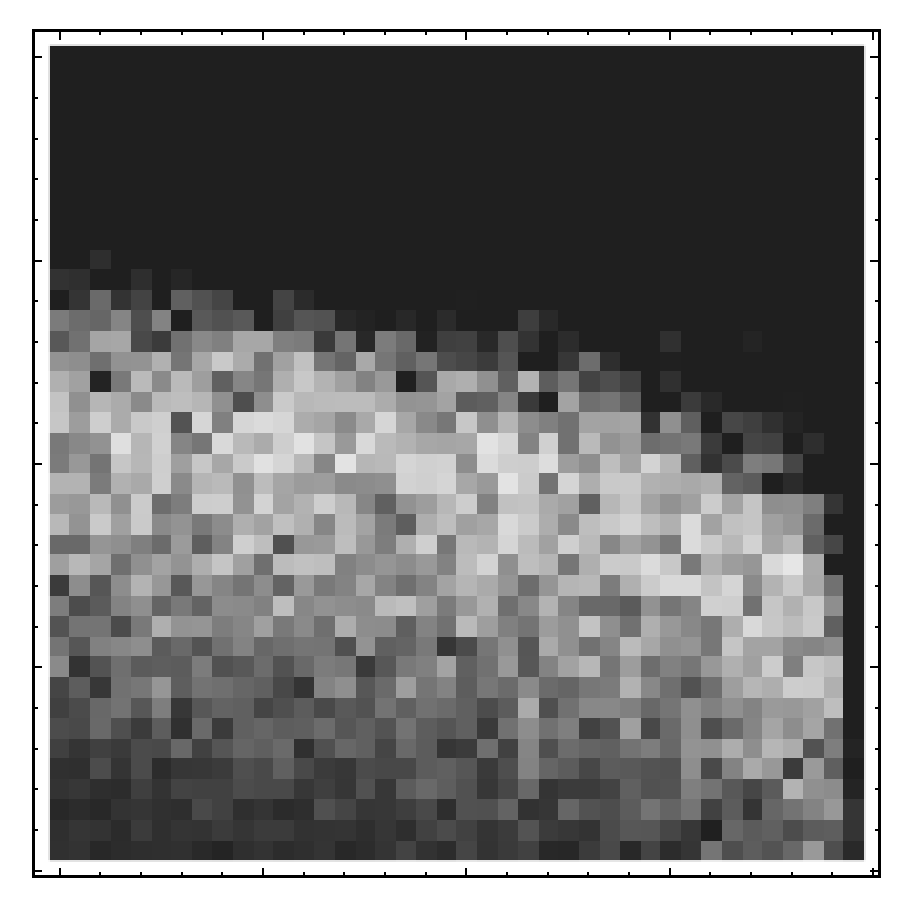
\includegraphics[scale=0.25]{plots/simple/LF-20R10R-20T10-CIFAR-3.eps} \\ \hline
BReLU 
        & 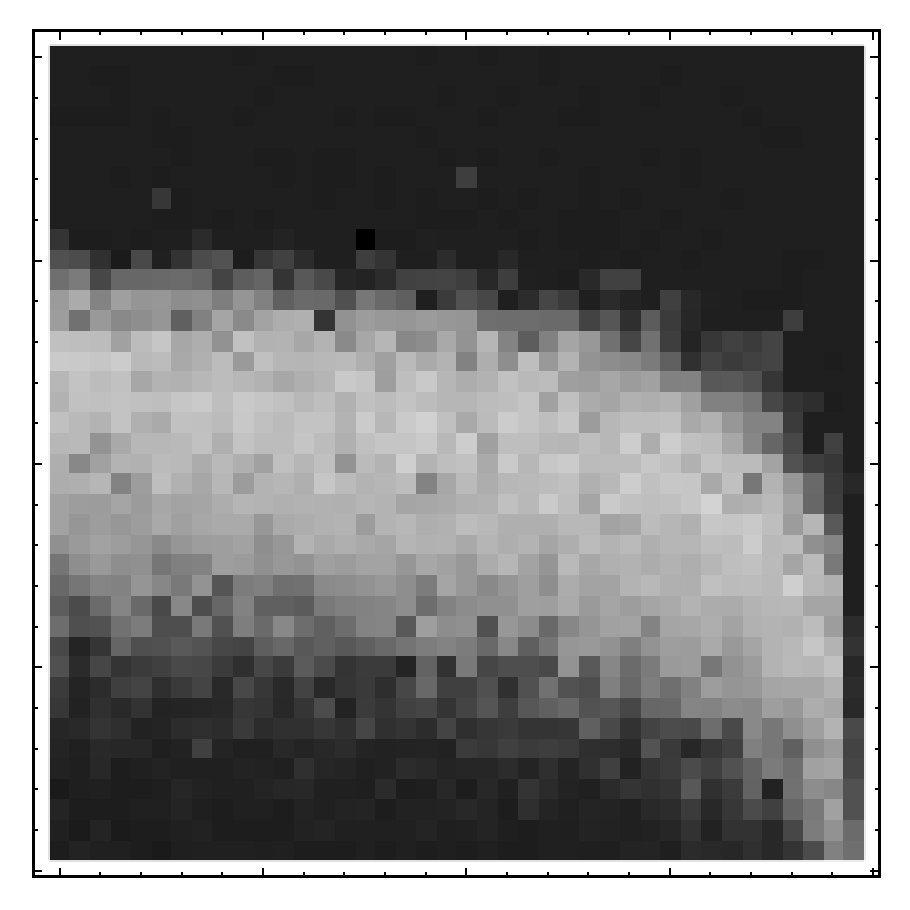
\includegraphics[scale=0.25]{plots/simple/LF-20BR10BR-20T10-CIFAR-1.eps}
        & 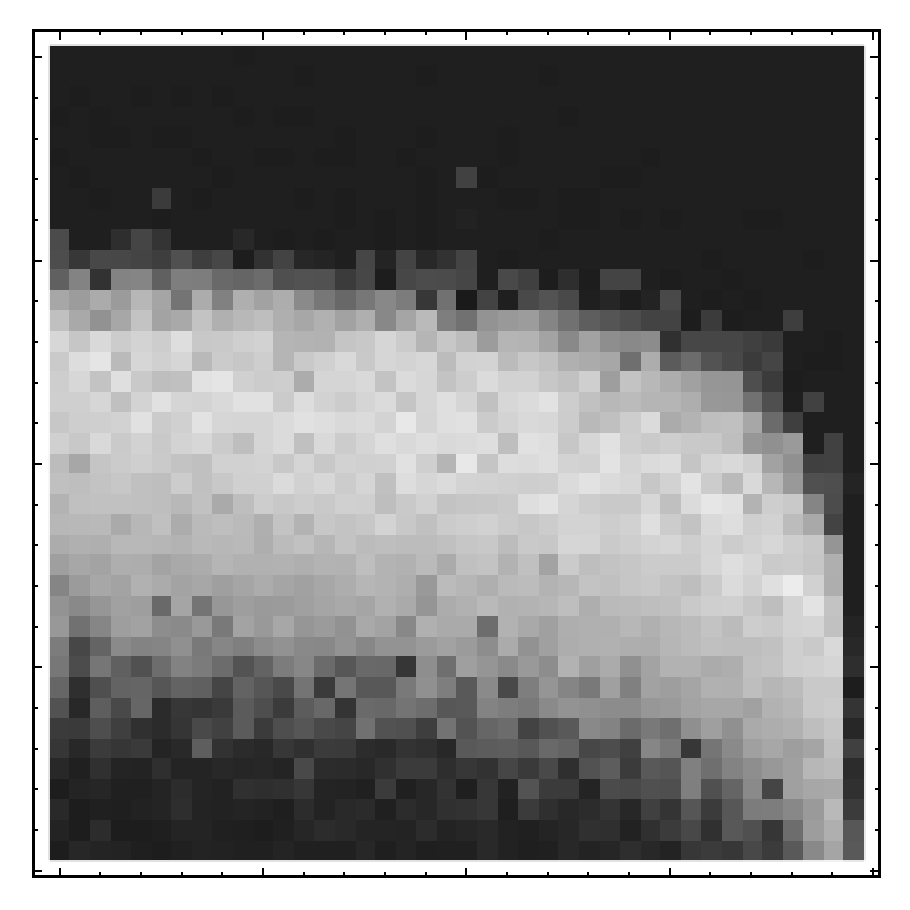
\includegraphics[scale=0.25]{plots/simple/LF-20BR10BR-20T10-CIFAR-2.eps}
        & 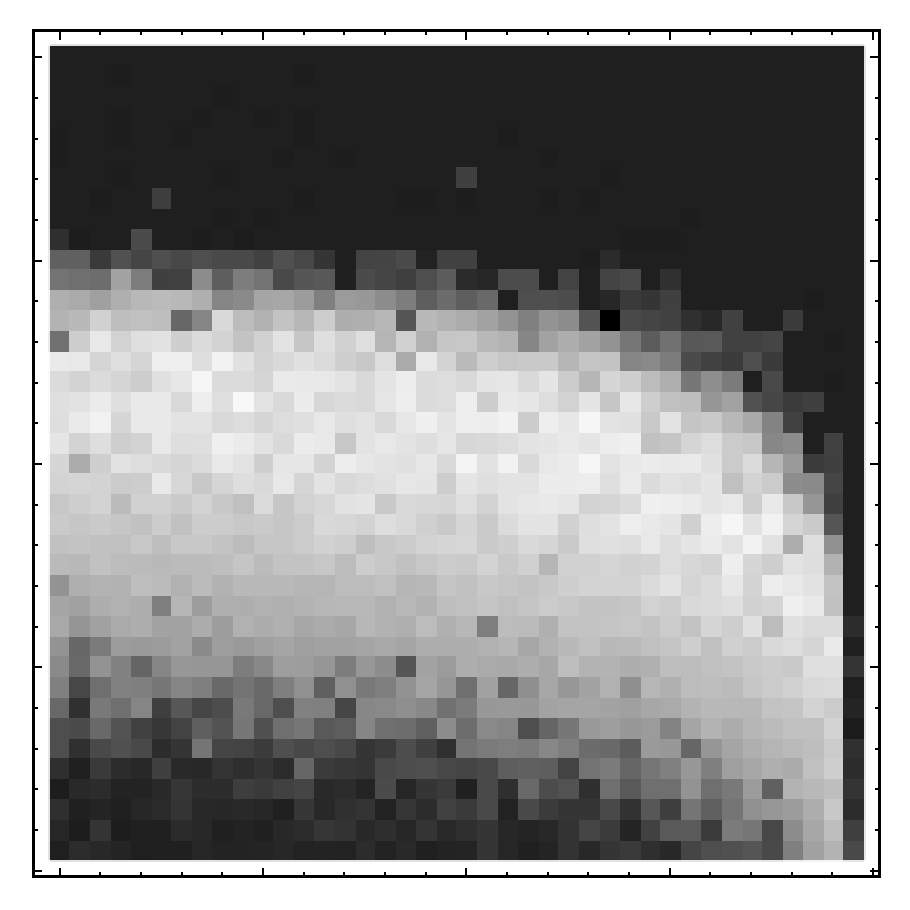
\includegraphics[scale=0.25]{plots/simple/LF-20BR10BR-20T10-CIFAR-3.eps} \\ \hline
\end{tabular}



Q: Should we introduce some notion of local variance / local
dependence on variation of parameters?  Chris: Hold the initialization
and ordering of data constant, and try the 40 x 4 experiments for a
ReLU subexperiment --- do we see the same ``splotchiness''?

``For practical purposes, BReLU is likely to be a good choice.''
Caveats.

Momentum-based gradient descent isn't that interesting.  Cite the
Simard 2003 results, who also found this.








Setup / detailed comments about what we do: 

+ Details of what is done: The hyperparameters divide up into two types:

+ Learning parameters: friction (correct to momentum), learning rate.
AMount of training data (sort of).  Other choices: Mini-batch size;
use of momentum based SGD.  Choice of training set.

+ Architecural parameters: weight initialization, structure of the
layers.  Activation function.  Stuff that's fixed: Cost function;
softmax.

+ Why these choices of 2d section, i.e., why these particular pairs?
It's worth pointing out that there are many other possibilities, and
many that are clearly worth investigating.  Our choices in this
particular paper were largely motivated by anothr project, in which
these particular questions arose as a practical matter affecting our
choice of hyper-parameters --- eg., the learning rate / frition
tradeoff, etc.  We believe that thse hoices are likely to be of broad
interest, but much more could be done.  A thorough examination would
be enormous.  SO to extent this is arbitrary, but it was motivated by
practically arising concerns.  COmputational expense; readability is
the real issue.


+ SHould we do classification accuracy?  Cost?  SOmething else?
Should make it easy to generate data, so anyone who cares can easily
compare and contrast.  (This means is that to some extent it doesn't
matter if we make the wrong choice.)  We will do at least one example
where we do both cost and classification accuracy.  We choose to focus
on cost because fundamentally this is what the SGD agorithmi is trying
to minimize.  Hoever for practial purposes classification accuracy of
course matters, and issues such as overfitting --- further work would
need to be done to addess these.  Note: One should also do it for
different cost functions.







2. Initialization of weights.

Architecture: 20 HU.

Activation functions: ReLU, sigmoid, tanh, TODO BReLU.

Training data: CIFAR.

Results: 2 types of movie. 

Claim: sigmoid is almost insensitive to initialization.

Claim: ReLU cares a lot about init.  THe product of the SDs matters a
lot.  ANd it's stochastic.




3. Learning rate 1 versus learning rate 2.

Architecture: 20 HU, 40 HU, 40+20 HU (fixed learning rate in final
layer).

Activation functions: sigmoid, ReLU, tanh, BReLU.

Training data: CIFAR.

Claim: Best rates not on diagonal.


4. Number of HU (single layer) versus size of training data

Architecture: single layer, + softmax.

Activation: sigmoid.

Training data: MNIST.


CLaim: Surprising how little data, or how littl HU are required.




Results

+ ??? To talk about: low-dimensional ``optimal'' manifold in
hyperparameter space.  Bengio's ICML2011 for algorithms on tuning
hyperparameters.

+ Obviously 3d versions... hard to computationally.

(Note: In some sense, it's 2+1 dimension, because we're actually
looking over training time.  We do Not look to saturate, i.e., to
get to optimal performance.  So the results are more about how quickly
we're learning, not asymptotic capacity.  Add a caveat: in fact,
almost noone ever does this.  One of the lessons of recent work is
that there's much more benefit to going to long training times than
people previously thought, with a suitable schedule of annealing.)







Nonlearities we want: sigmoid.  Tanh.  ReLU.  BReLU.

Data sets: CIFAR.  MNIST.

Weight initialization: 1/sqrt n.  10 / sqrt n.

Bias: 0 and 1.

Architectures.  20 neurons. 40 neurons.  20+40 neurons.  For 40 and
20+40 neurons, CIFAR only, one weight initialization only.

Averaging: Don't do any averaging for experiments.

List of desirable properties for nonlinearities.  Discuss.  It's a
tentative list, but did lead to BReLUs.  It's a first cut, Softplus
also has many of these properties, it would be interesting to explore
more systematically.


+ Weight initization doesn't matter for sigmoids, but it does for ReLUs.

+ Sample the space of hyper-parameters, then try to learn the manifold
of optimal hyper-parameters.

+ Mini-batch size.

FUTURE POSSIBILITIES: CO might do a Nesterov experiment?  SoftPlus.

XXX --- adaptive hyper-parameters?  Annealing?  Etc.

\subsection*{Bevelled Rectified Linear Units}

As part of our investigations we were led to introduce a new type of
activation function for an artificial neuron.  As seen above, this
activation function performed extremely well, and so it seems to be of
some independent interest to record here the heuristic considerations
which led to this activation function.

What's a good neural activation function look like?  Well,
heuristically you'd think it might ahve these properties: XXX.  Why
the conventional functions fail.  Recent work on ReLU in particular.
Potential shortcomings of ReLU.  We tried the following: BReLU.  As
we'll see below, we get surprisingly good results that seem to avoid
some of the problems with ReLU. (Mention Softplus with a citation).
Future work: XXX.  Of course, this isn't an actual argument, but it
does suggest that future investigations in this line may be
profitable.

\subsection*{Conclusion}

CHECK: PLoS One guidelines on conclusions.

OBSERVATION / RELATION TO PRIOR WORK: Over the past few years there's
been a lot of work using GPUs [refs] and cluster s[ refs] to train
neural networks.  Most of this work has focused on training larger and
deeper networks, for more epochs than before, to get superior
performance.  Our work demonstrates a dual strategy: instead of using
the increased comp power to train one or a few very large networks, we
use it to train very large numbers of relatively simple networks.  We
believe this dual strategy can be important to

+ LImit of the technique: These are only preliminary results.  Really
you want a much more comprehensive investigation.  It is even
possible, a priori, that there are no simple, esasily visualizable
rules of thumb to discover!  However, we believe it is worth at least
investigating the possibility, and our preliminary results suggest
that there is a surprisingly simple struture underlying regions of
hyperparameter space

+ Fun idea: AN atlas / periodic table of neural nets.  Would contain
lots of heuristics, and lots of failed heuristics that seem plausile
(but with disproofs).  Supprting evidence: lots and lots of videos.
Hundreds / thousands.

+ THe lower dimensional manifold: the parameters which are optimal in
hyperparameter space.


Glorot, Bngio et al: They found ReLU worked better than softplus in
deep networks.  How to reconcile with our results?

% Do NOT remove this, even if you are not including acknowledgments
\section*{Acknowledgments}

Thanks to David Dalrymple and Jen Dodd for helpful discussions.

%\section*{References}
% The bibtex filename
\bibliography{cifar}

\section*{Figure Legends}
%\begin{figure}[!ht]
%\begin{center}
%%\includegraphics[width=4in]{figure_name.2.eps}
%\end{center}
%\caption{
%{\bf Bold the first sentence.}  Rest of figure 2  caption.  Caption 
%should be left justified, as specified by the options to the caption 
%package.
%}
%\label{Figure_label}
%\end{figure}


\section*{Tables}
%\begin{table}[!ht]
%\caption{
%\bf{Table title}}
%\begin{tabular}{|c|c|c|}
%table information
%\end{tabular}
%\begin{flushleft}Table caption
%\end{flushleft}
%\label{tab:label}
% \end{table}

\end{document}
